\documentclass[a4paper,12pt]{article}
\usepackage[polish]{babel}
\usepackage[utf8]{inputenc}
\usepackage[T1]{fontenc}
\usepackage{tabularx}
\usepackage{amssymb}
\usepackage{amsmath}
\usepackage{latexsym}
\usepackage{graphicx}
\usepackage{fancyhdr}
\usepackage{chngpage}
\usepackage{enumerate}
\usepackage{enumitem}
\usepackage{listings}
\usepackage{geometry}
\usepackage{xcolor}
\linespread{1.5}
\pagestyle{fancy}
\geometry{lmargin=3.5cm, rmargin=2.5cm, bmargin=3cm, tmargin=3cm}

\lhead{}

\title
{
	\Large
	Akademia Górniczo-Hutnicza im. Stanisława Staszica \\ w Krakowie \\
	\vspace{10 mm}
	
\includegraphics[scale=0.8]{gfx/agh.jpg} \\
	\textbf{ System wykrywania podobieństw kodów źródłowych w projektach studenckich } \\
	Praca dyplomowa \\
	\vspace{10 mm}
}
\author
{
	\vspace{10 mm}
	Jarosław Szczęśniak \\
	Promotor: dr inż. Darin Nikolow
	\vspace{10 mm}
}

\begin{document}

\definecolor{light-gray}{gray}{0.95}
\lstdefinestyle{customjava}{
  backgroundcolor=\color{light-gray},
  numbers=left,
  numbersep=10pt,
  belowcaptionskip=1\baselineskip,
  breaklines=true,
  frame=L,
  xleftmargin=\parindent,
  language=Java,
  showstringspaces=false,
  basicstyle=\footnotesize\ttfamily,
  keywordstyle=\bfseries\color{green!40!black},
  commentstyle=\itshape\color{purple!40!black},
  identifierstyle=\color{blue},
  stringstyle=\color{orange},
}

\lstset{escapechar=@,style=customjava}

\renewcommand{\labelitemi}{$\bullet$}
\renewcommand{\labelitemii}{$\circ$}
\renewcommand{\labelitemiii}{\tiny$\blacksquare$}
\renewcommand{\labelitemiv}{$\diamond$}

\maketitle

\pagebreak

\tableofcontents

\newpage

\section{Wstęp}

\section{Cel i zakres prac}

Celem pracy jest zbudowanie systemu, który będzie wspomagał wykrywanie podobieństw w danych kodach źródłowych. Docelowym zagadnieniem z jakim ma zmierzyć się system jest porównywanie kodów źródłowych napisanych w języku Asembler.

Osiągnięcie celu głównego wymaga zrealizowania szeregu celów cząstkowych:
\begin{itemize}
\item zapoznanie się z dostępnymi metodami porównywania tekstu
\item zdefiniowanie języka wewnętrznego:
\begin{itemize}
	\item symboli leksykalnych
	\item gramatyki języka
\end{itemize}
\item implementacja co najmniej jednej metody porównywania
\item dostarczenie aplikacji analizującej kod źródłowy
\item dostarczenie środowiska do porównywania kodów źródłowych
\item dostarczenie przykładowych programów w języku wewnętrznym
\end{itemize}

Istnieje kilka skutecznych metod porównywania tekstu, poczynając od najprostszej i zarazem najmniej efektywnej metody brute-force, poprzez szybsze funkcje wykorzystujące zróżnicowane metody (np. funkcje hashujące), do algorytmów wykorzystujących deterministyczne automaty skończone.

Jednak w przypadku porównywania kodów źródłowych programów komputerowych problem staje się dużo bardziej złożony i zwykłe porównywanie tekstu nie jest najbardziej efektywną metodą, na której należy polegać \cite{arwin2006}. Najbardziej popularna klasyfikacja metod służących do wykrywania plagiatów kodów źródłowych uwzględnia sześć różnych podejść, skupiających się na\cite{roycordy2007}:
\begin{itemize}
\item tekscie - metoda bardzo szybka, ale może być łatwo oszukana poprzez zmianę nazw identyfikatorów i funkcji,
\item tokenach - większośc systemów opiera sie na tej metodzie, sposób działania taki sam jak podczas porównywania tekstu, jednak uniezależniony od identyfikatorów, komentarzy i białych znaków,
\item drzewach składniowych - pozwala na porównywanie kodów na wyższym poziomie, umożliwiając porównanie całych sekwencji kodu, np. wyrażeń warunkowych, czy funkcji,
\item Program Dependecy Graphs (PDGs) - inaczej zwane również multigrafami - grafy skierowane, które dokładnie odwzorowują logikę i przepływ programu, bardzo złożone i czasochłonne,
\item metrykach - wykorzystanie funkcji oceny na podstawie częstości występowania pewnego fragmentu kodu (np. pętli, wywołań funkcji, ilość wykorzystanych zmiennych), niezbyt skuteczna metoda, ponieważ dwa kody wykonujące całkowicie różne rzeczy mogą mieć tą samą ocenę,
\item hybrydzie - połączenie dowolnych dwóch powyższych metod.
\end{itemize}

W swojej pracy zdecydowałem się na podejście do problemu pod różnymi kątami i wykorzystanie kilku dostępnych metod.

Oprócz sposobów wymienionych powyżej istnieje jeszcze miara odmienności napisów (także odległość edycyjna, ang. ,,edit distance'' lub ,,Levenshtein distance''), zaproponowana przez Vladimira Levenshtein'a w 1965 roku\cite{editdistance}. Jest ona skutecznie wykorzystywana w rozpoznawaniu mowy, analizie DNA, korekcie pisowni, oraz w rozpoznawaniu plagiatów.

Z tego względu miara odmienności napisów wydaje się idealnym sposobem na zaimplementowanie metody wykrywającej plagiaty na podstawie porównywania tekstu i tokenów.

Na tym jednak rola odległości Levenshtein'a się nie kończy. Ponieważ porównanie samego tekstu nie jest najbardziej skutecznym sposobem na wykrywanie plagiatów w kodach źródłowych. Większy sens i sposób na uzyskanie największej dokładności w porównywaniu mają metody skupiające się wokół grafów i drzew (które są szczególnymi przypadkami grafu).

Izomorfizm grafów (a także drzew) jest wykorzystywany do sprawdzania podobieństwa grafów. Grafy A i B nazywami izomorficznymi wtedy, gdy istnieje bijekcja zbioru wierzchołków grafu A na zbiór wierzchołków grafu B. Innymi słowy oznacza to, że grafy A i B są takie same, jednak poddane pewnej permutacji wierzchołków. Rozstrzygnięcie izomorficzności dwóch grafów jest problemem klasy NP.

\begin{figure}[h!]
\centering
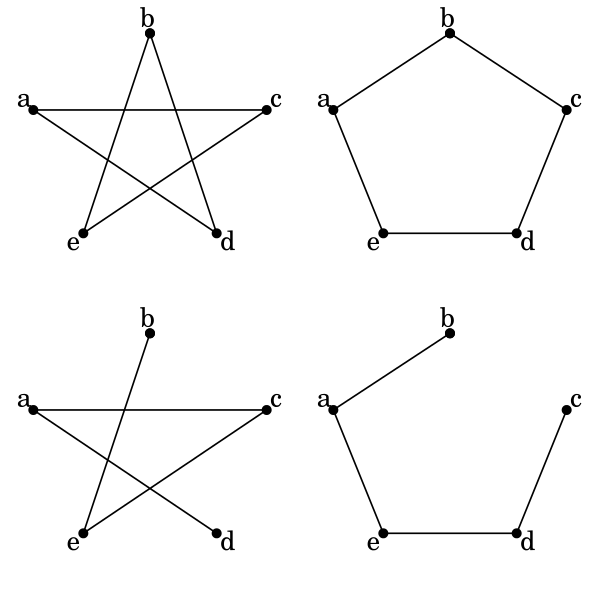
\includegraphics[scale=0.5]{gfx/isomorphism.png}
\caption{Grafy położone obok siebie są izomorficzne}
\end{figure}

Okazuje się, że odległość edycyjna jest z powodzeniem wykorzystywana w badaniu izomorficzności grafów i to wykorzystam ją jako kolejną metodę do wykrywania podobieństw pokrywającą porównywanie drzew składniowych (czyli grafów).

\newpage

\section{Teoria kompilacji}

Kompilator to program, który tłumaczy kod źródłowy na kod wynikowy. Składa się on z dwóch głównych etapów - analizy i syntezy.

Etap analizy składa się z trzech etapów pośrednich - analizy leksykalnej, składniowej i semantycznej. Polega on na rozłożeniu kodu źródłowego na czynniki składowe oraz na budowie jego reprezentacji pośredniej.

Ten właśnie etap wydaje się być odpowiednim procesem, dzięki któremu można będzie wykonać porównanie dwóch kodów źródłowych na odpowiednio wysokim, abstrakcyjnym poziomie, aby uniezależnić się od wykorzystywanego nazewnictwa lub organizacji i kolejności zdefiniowanych instrukcji w kodach źródłowych.

Język formalny to podzbiór zbioru wszystkich wyrazów nad skończonym alfabetem. Język formalny jest podstawowym pojęciem w informatyce, logice matematycznej i językoznawstwie. Aby zdefiniować język formalny musimy najpierw zdefiniować jego alfabet, składający się z symboli. Ciągi symboli nazywamy napisami, a dowolny zbiór tych ciągów to język formalny.

\subsection{Symbole}

Symbole leksykalne to abstrakcyjne ciągi znaków, które definiowane są podstawie określonych przez analizator reguł i przekazywane do dalszych etapów analizy. Reguły, według których są one definiowane, budowane są najczęściej z wyrażeń regularnych. Z symbolami leksykalnymi skojarzona jest też wartość leksykalna.
\\ \\
\begin{figure}[h!]
\centering
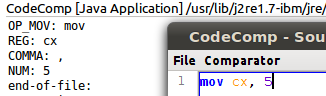
\includegraphics[scale=0.8]{gfx/tokens.png}
\caption{Przykład przedstawiający pewne wyrażenie oraz wynik działania parsera w postaci listy tokenów i ich wartości}
\end{figure}

Symbole, których używany najczęściej to litery lub cyfry. Alfabet jest to niepusty zbiór, składający się ze skończonej liczby symboli. Przykładem alfabetu, może być alfabet języka polskiego lub alfabet Morse’a.

Napis jest to skończony ciąg symboli, które należą do podanego alfabetu. Długość napisu oznaczamy jako |n| i jest to ilość symboli w napisie ,,n’’, przykładowo długość |tekst| wynosi 5.

Prefiksem napisu nazywamy pewną liczbę symboli rozpoczynających napis. Sufiksem nazywamy pewną liczbę symboli kończących napis. 

Język jest dowolnym zbiorem napisów ustalonym nad pewnym okreśłonym alfabetem. Językiem może być zbiór pusty, zbiór zawierający pusty napis lub pewien podzbiór ze zbioru wszystkich łańcuchów nad określonym alfabetem.

\subsection{Wyrażenia regularne}

Wyrażenia regularne to specyficzne wzorce, które umożliwiają zwięzłe i elastyczne sposoby wyszukiwania dopasowań ciągów tekstu, poszczególnych znaków lub wzorców znaków.

W tej pracy wyrażenia regularne wykorzystane zostaną tylko w jednym miejscu - w analizatorze leksykalnym. Dzięki nim zdefiniowane zostaną odpowiednie wzorce, które wychwycą w podanym kodzie źródłowym białe znaki, zwykłe znaki oraz liczby, z których zbudowane są zmienne, funkcje i identyfikatory.

\subsection{Gramatyka}

To, co definiuje leksemy, to zestaw reguł określonych na podstawie specyfikacji języka programowania, czyli gramatyki.

Obecnie najczęściej stosuje się wyrażenia regularne do zdefiniowania reguł. Określają one zestaw możliwych sekwencji, które są użyte do zbudowania konkretnych leksemów.

W niektórych językach programowania kod dzieli się na bloki za pomocą par symboli (np. ,,\{‘’ i ,,\}’’), które razem z innymi białymi znakami również opisane są za pomocą leksemów, lecz nie są brane pod uwagę podczas dalszych etapów analizy.

\subsection{Analiza leksykalna}

Analiza leksykalna służy do dzielenia strumienia znaków wejściowych na grupy (symbole), do których dopasowywane są pewne sekwencje (leksemy) na podstawie reguł (wzorców), w celu przekazania ich do dalszego etapu analizy. Leksem to abstrakcyjna jednostka leksykalna, która może obejmować słowa kluczowe, identyfikatory, etykiety, operatory, separatory, komentarze lub inne symbole specjalne.

\subsubsection{Skaner}

Skaner, czyli podstawowa część analizatora leksykalnego, zajmuje się głównym etapem analizy. Posiada on informacje na temat sekwencji znaków, które mogą być wykryte i zapisane jako symbole.

W wielu przypadkach pierwszy znak, który nie jest znakiem białym może posłużyć do dedukcji, z jakiego rodzaju symbolem mamy do czynienia (longest-match rule). W przypadku bardziej skomplikowanych języków potrzebna jest możliwość cofania się do wcześniej wczytanych znaków.

Skaner wczytuje kolejne znaki ze strumienia wejściowego i klasyfikuje je według reguł w symbole leksykalne, które następnie przekazywane są do analizy składniowej. Jako jednostka rozpoczynająca analizę i wczytująca tekst źródłowy może służyć również jako filtr, który pomija pewne elementy, takie jak np. komentarze, białe znaki lub znaki nowego wiersza.

Możliwe jest i czasem konieczne napisanie własnego analizatora, aczkolwiek jest to zwykle zbyt skomplikowane, czasochłonne i nieopłacalne. Z tego względu analizatory, zwane lekserami, zwykle generowane są za pomocą specjalnych narzędzi, które przyjmują na wejściu wyrażenia regularne, które opisuję wymagane symbole leksykalne.

Jednym z najbardziej popularnych generatorów analizatorów leksykalnych jest program Flex\cite{flex}, który posiada swoją implementację w Javie o nazwie JFlex\cite{jflex}.

To właśnie JFlex został wykorzystany do wygenerowania skanera na podstawie gramatyki, która składa się z trzech części: kodu użytkownika, zdefiniowanych za pomocą wyrażeń regularnych tokenów oraz definicji reguł leksykalnych.

\subsection{Analiza składniowa}

Analiza składniowa to proces analizy tekstu, złożonego z symboli, którego celem jest wyklarowanie jego struktury gramatycznej na podstawie zdefiniowanej gramatyki.

\subsubsection{Parser}

Jest to komponent, który wykonując analizę składniową, sprawdza jej poprawność i tworzy pewną strukturę danych (często tzw. drzewo składniowe), składającą się z symboli wejściowych. Korzysta z analizatora leksykalnego, który zaopatruje go w zestaw symboli leksykalnych zbudowanych ze strumienia wejściowego. Innymi słowy parser analizuje kod źródłowy i tworzy jego wewnętrzną reprezentację.

\subsubsection{Typy parserów}

Zadaniem parsera jest określenie czy i w jaki sposób symbole leksykalne mogą być przekształcone na symbole gramatyczne. Istnieją dwa sposoby, dzięki którym osiągniemy rządany efekt:
\begin{itemize}
	\item parsowanie zstępujące (top-down) -- polega na znalezieniu symboli wysuniętych najbardziej na lewo przeszukując drzewo składniowe z góry na dół.
	\item parsowanie wstępujące (bottom-up) -- polega na sprawdzeniu począwszy od słowa wejściowego i próbie redukcji do symbolu startowego, analizę zaczynamy od liści drzewa posuwając się w kierunku korzenia.
\end{itemize}

Do wygenerowania parsera opierającego się na metodzie zstępującej wykorzystany został program BYACC/J\citep{byaccj}. Jest to rozszerzenie generatora BYACC stworzonego na uniwersytecie Berkeley\cite{byacc}, który na podstawie gramatyki opisanej w notacji zbliżonej do BNF (Backus Normal Form)\cite{BNF} generuje parser w języku Java.

\newpage

\section{Wprowadzenie do Asemblera}

Historia asemblera sięga lat 50. tych XX wieku, kiedy powstał pierwszy asembler stworzony przez niemieckiego inzyniera Kondrada Zuse. Stworzył on pierwszy układ elektromechaniczny, który na podstawie wprowadzanych przez użytkownika rozkazów i adresów tworzył taśmę perforowaną zrozumiałą dla wyprodukowanego przez niego komputera Z4.

Asembler jest to program, który tłumaczy kod źródłowy, napisany w języku niskopoziomowym, na kod maszynowy. Proces ten nosi nazwę asemblacji. 

Język asembler (ang. \textbf{assembly language}) jest to język programowania komputerowego, należący do grupy języków niskopoziomowych. Oznacza to, że jedna instrukcja języka asembler odpowiada dokładnie jednej instrukcji kodu maszynowego, przeznaczonej do bezpośredniego wykonania przez procesor.

Istnieje kilka różnych implementacji języka asembler. Składnia każdego z nich jest zależna od architektury konkretnego procesora. Najbardziej popularnym obecnie asemblerem jest Asembler x86.

\subsection{Instrukcje}

Każda instrukcja języka asembler jest reprezentowana przez łatwy do zapamiętania tzw. mnemonik, który w połączeniu z jednym lub wieloma argumentami tworzy kod operacji (ang. \textbf{opcode}).

Specyfikacja i format operacji zależy architektury procesora (ang \textbf{ISA - Instruction Set Architecture}), która definiuje listę dostępnych rozkazów procesora, typów danych, rejestrów, obsługę wyjątków i przerwań.

Argumentami operacji mogą być (w zależności od architektury): rejestry, wartości stosu, adresy w pamięci, porty I/O, itp.

Lista typów operacji składa się z operacji:
\begin{itemize}
\item arytmetycznych
\item logicznych
\item transferowych
\item skokowych
\item różnych
\end{itemize}

Asembler x86 posiada dwie podstawowe składnie: Intel i AT\&T. Składnia Intel jest dominującą w systemach DOS i Windows, natomiast AT\&T w systemach Unixowych\cite{asm_syn}.

\begin{figure}[h!]
\centering
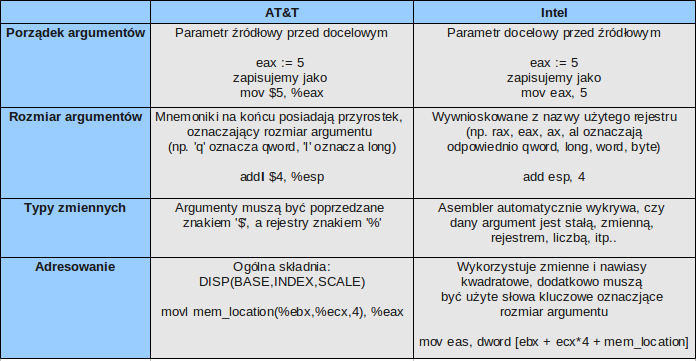
\includegraphics[scale=0.6]{gfx/asm_syn_diff.png}
\caption{Główne różnice pomiędzy składniami Intel i AT\&T\cite{asm_syn}}
\end{figure}

\subsection{Typy danych}

Typy danych w języku asembler są ściśle związane z pojęciem dyrektyw.

Dyrektywy to instrukcje, które definiują typ danych, ich rozmiar, zasięg i alokują je w pamięci.

\\
\begin{center}
\begin{tabular}{|c|c|}
\hline 
Dyrektywa & Typ danych \\ 
\hline 
DB & Byte (8b) \\ 
\hline 
DW & Word (16b) \\ 
\hline 
DD & Doubleword (32b) \\ 
\hline 
DQ & Quadword (64b) \\ 
\hline 
DT & Ten bytes (80b) \\ 
\hline 
\end{tabular} 
\end{center}
\\

Typy danych dzielimy na dwie kategorie: numeryczne i alfanumeryczne. W skład danych numerycznych wchodzą liczby całkowite i zmiennoprzecinkowe. Kody alfanumeryczne wykrzystywane są do przechowywania napisów.

\subsection{Adresowanie}

Adresowanie określa sposób, w jaki odnosimy się do adresu w pamięci, który określa położenie argumentów rozkazu.

\textbf{Adresowanie natychmiastowe}

Adresowanie natychmiastowe (ang. \textbf{immediate addressing}) to najprostsza metoda adresowania, w którym zamiast podawania adresu operandu jego wartość podana jest jawnie w instrukcji. Ten sposób adresowania jest możliwy tylko dla stałych.

\begin{lstlisting}
mov eax, 5
\end{lstlisting}

\textbf{Adresowanie bezpośrednie}

Adresowanie bezpośrednie (ang. \textbf{direct addressing}) polega na podaniu w instrukcji adresu pamięci, w którym znajduje się operand. W ten wygodny sposób można wykorzystać używając zmiennych globalnych, których adres nie zmienia się w trakcie działania programu.

\begin{lstlisting}
mov eax, [0xFFFFFF]
\end{lstlisting}

\textbf{Adresowanie rejestrowe}

Adresowanie rejestrowe (ang. \textbf{register addressing}) wykorzystuje rejestr, w którym operand jest przechowywany.

\begin{lstlisting}
mov eax, ebx
\end{lstlisting}

\textbf{Adresowanie pośrednie rejestrowe}

W adresowanie pośrednie rejestrowe (ang. \textbf{indirect addressing mode}) adres operandu zapisany jest w jednym z rejestrów. Oznacza to, że rejestr staje się wskaźnikiem do wartości operandu.

\begin{lstlisting}
mov eax, [ebx]
\end{lstlisting}

\textbf{Adresowanie indeksowe}

Adresowanie indeksowe (ang. \textbf{indexed addressing}) polega na dodaniu do wartości rejestru, w którym znajduje się adres operandu, tzw. offsetu, czyli przesunięcia względem początku bloku danych.

\begin{lstlisting}
mov eax, [0xFFFFFF + ebx * 1]
\end{lstlisting}

\textbf{Adresowanie indeksowe z wartością bazową}

Adresowanie indeksowe z wartością bazową (ang. \textbf{based indexed addressing}) występuje tylko w niektórych rodzajach procesorów. Polega na obliczeniu adresu operandu poprzez zsumowanie wartości dwóch rejestrów i dodaniu opcjonalnego przesunięcia. Pierwszy rejestr zawiera adres podstawowy, drugi indeks. Indeks mnożony jest przez rozmiar słowa, a do całości dodawane jest przesunięcie.

\begin{lstlisting}
mov eax, [0xFFFFFF + ebx + ecx * 1]
\end{lstlisting}

\subsection{Lista instrukcji}

List instrukcji to najważniejszy element wykorzystywany w parserze. Dokładne i odpowiednie zdefiniowanie listy jest kluczowe podczas rozpoznawania tokenów na podstawie kodu źródłowego i stworzenia poprawnego grafu.

\begin{itemize}
\item Operacje arytmetyczne bez lub z 1 argumentem:
	\begin{itemize}
	\item aaa
	\item daa
	\item inc $dest$
	\item dec $dest$
	\end{itemize}
\item Operacje arytmetyczne z dwoma argumentami:
	\begin{itemize}
	\item adc $src, dest$
	\item add $src, dest$
	\item cmp $src_1$, $src_2$ 
	\item {[i]}div $src, dest$
	\item {[i]}mul $src, dest$
	\item sbb $src, dest$
	\item sub $src, dest$
	\item sa[lr] $number, dest$
	\item rc[lr] $number, dest$
	\item ro[lr] $number, dest$ 
	\end{itemize}
\item Operacje logiczne bez lub z jednym argumentem:
	\begin{itemize}
	\item nop 
	\item not $dest$
	\item neg $dest$
	\end{itemize}
\item Operacje logiczne z dwoma argumentami:
	\begin{itemize}
	\item and $src, dest$
	\item or $src, dest$
	\item xor $src, dest$
	\item sh[rl] $dest, src$
	\item test $src_1$, $src_2$
	\end{itemize}
\item Operacje transferu bez lub z jednym argumentem:
	\begin{itemize}
	\item clc
	\item cld
	\item cli
	\item cmc
	\item pop[ad]
	\item pop[f] $dest$
	\item push[ad]
	\item push[f] $src$
	\item st[cdi]
	\end{itemize}
\item Operacje transferu z dwoma argumentami:
	\begin{itemize}
	\item mov $src, dest$
	\item movzx $src, [dest]$
	\item in $src, dest$
	\item out $src, dest$
	\item xchg $dest, dest$
	\end{itemize}
\item Operacje skoku:
	\begin{itemize}
	\item call $dest$
	\item jmp $dest$
	\item j$Warunek$ $dest$
	\item ret[fn] $number$
	\end{itemize}
\item Operacje różne:
	\begin{itemize}
	\item bswap $reg$
	\item int $src$
	\item lea $dest, src$
	\item nop
	\end{itemize}
\end{itemize}

\newpage

\section{Metody porównywania}

Każda z opisanych metod posiada szereg cech ją charakteryzujących. Są to:
\begin{itemize}
\item faza preprocesingu - przygotowania danych wejściowych do analizy
\item ilość potrzebnej pamięci dodatkowej
\item złożoność czasowa - ilość wykonywanych operacji względem ilości danych wejściowych
\end{itemize}

\subsection{Porównywanie tekstu}

\subsubsection{Algorytm brute-force}

Metoda brute -- force, w teorii, jest najskuteczniejszą metodą, ponieważ sukcesywnie sprawdza wszystkie możliwe kombinacje w poszukiwaniu rozwiązania problemu. W praktyce jednak, algorytmy oparte na tej metodzie są niezwykle nieoptymalne, ze względu na czas wykonywania, przez co są rzadko stosowane.

Algorytm polega na sprawdzeniu wszystkich pozycji w tekscie pomiędzy znakiem $0$ i $n-m$, gdzie $m$ to długość poszukiwanego wzorca, a $n$ to długość tekstu. Algorytm weryfikuje, czy wzorzec zaczyna się na danej pozycji. Jeśli tak to pozycja elementu w tekscie zapisywana jest do bufora. Następnie przesuwa wskaźnik w prawo po każdej próbie. Jeśli na kolejnych pozycjach znajdują się wszystkie kolejne elementy z wzorca to do tablicy wynikowej przepisywany jest zawartość bufora. Algorytm może być wykonywany w dowolnym kierunku, od przodu lub od tyłu.

Metoda nie wymaga żadnej fazy przed rozpoczęciem wykonywania algorytmu. Ze względu na charakter metody wymaga dodatkowego miejsca w pamięci. Złożoność czasowa wynosi $O(m*n)$, a ilość operacji potrzebna do wykonania algorytmu wynosi $2n$.

\pagebreak

Przykładowy kod źródłowy algorytmu brute -- force, wyszukującego określony wzorzec w podanym tekście:
\begin{lstlisting}
void BF(char *x, int m, char *y, int n) {
   int i, j;
   for (j = 0; j <= n - m; ++j) {
      for (i = 0; i < m && x[i] == y[i + j]; ++i);
      if (i >= m)
         OUTPUT(j);
   }
}
\end{lstlisting}

\newpage

\subsubsection{Algorytm Boyer-Moore}

Algorytm Boyer-Moore został stworzony w 1977 roku i do tej pory uważany jest za najbardziej optymalny algorytm poszukiwania wzorca w tekscie. Dowodem na to jest fakt, że algorytm ten jest zaimplementowany w większości najbardziej popularnych aplikacji z opcją ,,Znajdź’’ lub ,,Zamień’’.

Algorytm szuka danego wzorca w teksćie porównując kolejne znaki tekstu do wzorca, lecz w odróżnieniu od metody brute-force wykorzystuje informacje zebrane za pomocą fukcji preprocesujących, aby pominąć jak najwięcej znaków w tekście, które na pewno nie pasują do wzorca.

Procedura zaczyna się w miejscu k = n, w taki sposób, że początek wzorca P jest wyrównany do początku tekstu T. Następnie poszczególne znaki z P i T są porównywane począwszy od indeksu n w P i indeksu k w T, porusząjąc się od prawej do lewej strony wzorca P. Porównywanie trwa dopóki znaki w P i T nie są różne lub do momentu dotarcia do początku P (co oznacza, że znaleziono wystąpienie w tekście), a następnie indeks porównywania przesuwany jest w prawo o maksymalną wartość wskazywaną przez zdefiniowane reguły. Czynności są powtarzane do momentu sprawdzenia całego tekstu T.

Reguły przesuwania indeksu definiowane są za pomocą tabel tworzonych za pomocą funkcji preprocesujących.

\pagebreak

Przykład implementacji:
\begin{lstlisting}[h!]
public List<Integer> match() {
 List<Integer> matches = new LinkedList<Integer>();
 computeLast();
 computeMatch();

 int i = text.length() - 1;
 int j = pattern.length() - 1;
  while (i >= 0 && i < text.length()) {
   try {
    if (pattern.charAt(j) == text.charAt(i)) {
	if (j == 0) {
	 matches.add(i);
	 j = pattern.length() - 1;
    }
	j--; i--;
   } else {
    i -= Math.max(match[j], last[text.charAt(i)] 
       - text.length() + 1 + i);
    j = pattern.length() - 1;
   }
  } catch (Exception ex) { (...)  }
 }
 return matches;
}
\end{lstlisting}

\newpage

\subsubsection{Odległość Levenshtein'a}

Odległość Levenshtein'a - inaczej odległość edycyjna (ang. \textbf{edit distance}) - to metryka napisu, która określa różnicę pomiędzy dwiema sekwencjami znaków. Została wymyślona i zdefiniowana przez rosyjskiego naukowca Vladimira Levenshtein'a w 1965 roku.
Jej wynikiem jest minimalna ilośc operacji na pojedynczych znakach (wstawienia, usunięcia, podmiany) potrzebnej do zamiany jednego słowa w drugie.

\textbf{Definicja}

Odległośc Levenshtein'a pomiędzy napisami $a$ i $b$ określona jest wzorem $lev_{a,b}(|a|,|b|)$, gdzie:
\begin{center}
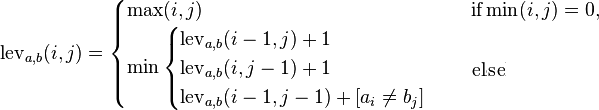
\includegraphics[scale=0.7]{gfx/levenshtein_def.png}
\end{center}

\textbf{Przykład}

Odległość edycyjna pomiędzy słowami $inżynier$ i $magister$ wynosi 6:
\begin{enumerate}
\item \textbf{i}nżynier $\rightarrow$ \textbf{m}nżynier
\item m\textbf{n}żynier $\rightarrow$ m\textbf{a}żynier
\item ma\textbf{ż}ynier $\rightarrow$ ma\textbf{g}ynier
\item mag\textbf{y}nier $\rightarrow$ mag\textbf{i}nier
\item magi\textbf{n}ier $\rightarrow$ magi\testbf{s}ier
\item magis\textbf{i}er $\rightarrow$ magis\textbf{t}er
\end{enumerate}

\pagebreak

\textbf{Cechy}

Odległość edycyjna posiada kilka cech, które mają zastosowanie w każdym przypadku i warto je wykorzystać w trakcie implementowania algorytmu:
\begin{itemize}
\item odległość jest zawsze conajmniej równa różnicy długości dwóch napisów
\item maksymalna wartość odległości jest równa długości dłuższego napisu
\item odległość jest równa zero wtedy i tylko wtedy, gdy napisy są identyczne
\item ogległość pomiędzy dwoma napisami jest nie większa niż suma ich odległości pomiędzy trzecim napisem
\end{itemize}

Odległość Levenshtein'a jest wykorzystana w technikach dopasowania przybliżonego, które polega na znalezieniu takich napisów, które w przybliżeniu pasują do wzorca. Techniki te znajdują zastossowanie w korektorach pisowni, systemach rozpoznawania znaków  (OCR - Optical Character Recognition) oraz w systemach do wykrywania plagiatów.

Głównym elementem w systemach wykrywania plagiatów jest zawsze graf. Może on posiadać postać drzewa, grafu skierowanego i nieskierowanego lub multigrafu. Stanowi on reprezentacje kodów źródłowych, które porównujemy. Aby ocenić, w jakim stopniu dwa kodu źródłowe są do siebie podobne, musimy sprawdzić w jakim stopniu podobne są do siebie dwa grafy.

Temat podobieństwa grafów jest istotnym elementem podczas badań w przestrzeni rozpoznawania wzorców. Możliwość określenia dokładnego podobieństwa pomiędzy grafami jest kluczowa, a odległość edycyjna stała się podstawą całego procesu \cite{ged}.

\newpage

\subsection{Izomorfizm grafu}

Problem izomorfizmu grafów polega na określeniu, czy dwa grafy są izomorficzne, czyli identyczne.

Poza praktycznym zastosowaniem w wielu różnych dziedzinach, zagadnienie to jest ciekawe i, z punktu widzenia teorii złożoności obliczeniowej, uznawane za jedno z niewielu problemów decyzyjnych należących do klasy NP, których rozwiązania nie można zweryfikować w czasie wielomianowym oraz jednym z dwóch problemów, których złożoność pozostaje nierozstrzygnięta\cite{np}.

Jednocześnie problem izomorfizmu dla szczególnych rodzajów grafów może być rozwiązany w czasie wielomianowm i w optymalny sposób. Te szczególne klasy grafów to:
\begin{itemize}
\item drzewo\cite{iso_tree}
\item graf planarny\cite{iso_planar}
\item graf przedziałowy\cite{iso_interval}
\item graf permutacji\cite{iso_perm}
\item niepełne drzewo rzędu k\cite{iso_ktree}
\item graf o ograniczonym stopniu\cite{iso_degree}
\item graf o ograniczonym genus (rodzaj topologiczny)\cite{iso_genus}
\end{itemize}

Izomorfizm grafów bada dokładną zgodność pomiędzy nimi, natomiast podczas wykrywania plagiatów zachodzi również potrzeba sprawdzenia, czy w danym kodzie źródłowym istnieje tylko pewna jego część (np. jedna funkcja), która występuje w drugim źródle.

Problem izomorfizmu grafu może być uogólniony do problemu izomorfizmu podgrafu, który można zastosować do rozwiązania wyżej opisanego problemu.

\pagebreak

\subsection{Izomorfizm podgrafu} 

Problem izomorfizmu podgrafu polega na określeniu, czy dla podanych grafów $G$ i $F$, istnieje taki podgraf grafu $G$, który jest izomorficzny z grafem $F$. Należy on do klasy problemów NP-zupełnych.

Grafem G nazywamy niepusty zbiór $V$ elementów $p$, zwanych węzłami, oraz zbiór $E$ składający się z różnych nieuporządkowanych par węzłów należących do $V$. Pary węzłów należące do $E$ nazywamy krawędziami.

Podgrafem grafu $G$ nazywamy graf, którego wszystkie węzły i krawędzie należą do grafu $G$. Graf $G_\alpha$ jest izomorficzny z podgrafem grafu $G_\beta$ wtedy i tylko wtedy, gdy istnieje zgodność w stosunku 1:1 pomiędzy zbiorami węzłów tego podgrafu i grafu $G_\alpha$, zachowująca sąsiedztwa węzłów\cite{ullmann}.

\subsubsection{Algorytm brute-force}

Algorytm brute-force to algorytm przeszukiwania w głąb i polega na znalezieniu wszystkich izomorficznych grafów $G_\alpha = (V_\alpha, E_\alpha)$ i podgrafów grafu $G_\beta = (V_\beta, E_\beta)$.
\\ \\
\textbf{Opis algorytmu}
\\ \\
Założenia\cite{ullmann}: \\
$p_\alpha \in V_\alpha$ \hspace{20} 
$q_\alpha \in E_\alpha$ \hspace{20} 
$p_\beta \in V_\beta$   \hspace{20}
$q_\beta \in E_\beta$ \\
$A = [a_{ij}]$ - macierz sąsiedztwa grafu $G_\alpha$ \\
$B = [b_{ij}]$ - macierz sąsiedztwa grafu $G_\beta$
$C = [c_ij] = M'(M'B')^T, gdzie T - transpozycja$
$M' = p_\alpha X p_\beta$ - macierz, której elementy przyjmują wartość 0 lub 1; każdy wiersz zawiera dokładnie jeden element o wartości 1 i żadna kolumna nie zawiera wiecej niż jeden element o wartości 1; może być wykorzystana podczas permutacji wierszy i kolumn macierzy $B$ w celu wyprodukowania macierzy $C$ \\
$F = \{ F_1, \ldots, F_i, \ldots, F_{p_\beta} \}$ - wektor przechowujący wykorzystane kolumny w trakcie działania algorytmu \\
$H = \{ H_1, \ldots, H_d, \ldots, H_{p_\alpha} \}$ - wektor przechowujący odległość od korzenia wybranej kolumny \\
$H_d = k$, jeżeli $k-ta$ kolumna znajduje się w odległości $d$ od korzenia
\\
Jeżeli twierdzenie:

$(\forall{i} \forall{j}) (a_{ij} = 1) \Rightarrow (c_ij = 1)$ \\
jest prawdziwe, to $M'$ określa izomorfizm pomiędzy $G_\alpha$ i podgrafem grafu $G_\beta$.
\\ \\
Pierwszym krokiem jest stworzenie $p_\alpha X p_\beta$ elementowej macierzy $M^0 = [{m^0}_{ij}]$, w której:
\\
${m^0}_{ij}$ \left\{
  \begin{array}{l l}\label{con}
    = 1, & \quad \text{gdy stopień $j-tego$ węzła grafu $G_\alpha$ $\geq$ stopniowi $i-tego$ węzła grafu $G_\alpha$}\\
    = 0, & \quad \text{w przeciwnym wypadku.}
  
  \end{array} \right.\]
\\ \\
Następnie, wykonujemy główną część algorytmu\cite{ullmann}:
\begin{enumerate}
\item{
$M = M^0, \ d = 1; \ H_1 = 0;$ \\
Dla każdego $i = 1, .., p_\alpha,$ ustaw $F_i = 0;$
}
\item{
Jeśli nie istnieje takie $j$, dla którego $m_{dj} = 1$ i $F_j = 0$ przejdź do kroku nr 7;\\
$M_d = M;$\\
Jeśli $d = 1$ to $k = H_1$, w przeciwnym wypadku $k = 0$
}
\item{
$k = k + 1;$\\
Jeśli $m_{dk} = 0$ lub $F_k = 1$ to przejdź do kroku nr 3;\\
dla każdego $j \neq k$ ustaw $m_{dj} = 0;$
}
\item{
Jeśli $d < p_\alpha$ to przejdź do kroku nr 6, w przeciwnym wypadku sprawdź warunek(0) i wypisz, jeśli znaleziono izomorfizm;
}
\item{
Jeśli nie istnieje $j > k$, dla którego $m_{dj} = 1$ i $F_j = 0$ to przejdź do kroku nr 7;\\
$M = M_d;$\\
przejdź do kroku nr 3;
}
\item{
$H_d = k$, $F_k = 1;$ $d = d + 1;$\\
przejdź do kroku nr 2;
}
\item{
Jeśli $d = 1$ to zakończ algorytm,\\
$F_k = 0;$ $d = d - 1$, $M = M_d$, $k = H_d$;\\
przejdź do kroku nr 5;
}
\end{enumerate}

\newpage

\subsubsection{Algorytm Ullmann'a}

% izomorfizm i edit distance

\newpage

\subsubsection{Algorytm VF2}

\cite{vf2}

\newpage

\section{Projekt systemu CodeComp}

W tym rozdziale przedstawiono opis aplikacji CodeComp, jej budowę wewnętrzną oraz sposoby instalacji i użycia.

\subsection{Architektura systemu}

Program składa się z kilku głownych pakietów: Comparator, Algorithm, Analyzer oraz GUI.

\begin{figure}[!h]
\centering
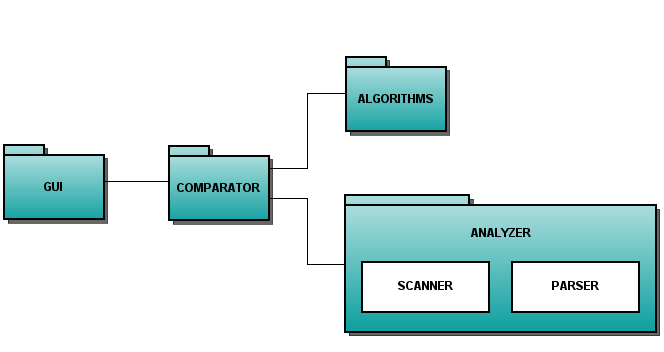
\includegraphics[scale=0.65]{gfx/packagediagram.png}
\caption{Diagram przedstawiający strukturę aplikacji}
\end{figure}

Comparator jest podstawowym, statycznym obiektem, który na wejściu pobiera kody źrodłowe programów porównywanych i przekazuje je do analizatora. Analizator zwraca nieskierowane grafy porównywanych kodów źródłowych, które w dalszym etapie przekazane są jako parametry algorytmu wybranej metody weryfikowania podobieństwa. 

Wynikiem działania komparatora jest procentowa wartość podobieństwa pomiędzy dwoma kodami źródłowymi oraz graficzna prezentacja miejsc identycznych w porównywanych źródłach.
\\ \\
Algorithm to pakiet, w którego skład wchodzi zestaw algorytmów porównywania tekstu oraz badania izomorficzności grafów. 

Algorytmy porównywania tekstu wykorzystane zostały do graficznego zaznaczania fragmentów identycznych w porównywanych kodach źródłowych. Na wejście przyjmują teksty kodów źródłowego w całości, następnie dzielą je na pojedyncze wyrazy i sprawdzają, czy dany wyraz z jednego kodu źródłowego znajduje się w dowolnym miejscu w drugim źródle. Wynikiem działania algorytmów porównywania tekstu jest lista identycznych wyrazów oraz ich położenie w obu źródłach.

Algorytm sprawdzania izomoriczności grafów przyjmuje na wejście dwa grafy skierowane i wykorzystuje algorytm VF2 do obliczenia dystansu pomiędzy nimi. Wynikiem jego działania jest wartość liczbowa oraz procentowa obliczonej odległości.
\\ \\
Analyzer to komponent, który zajmuje się etapem analizy z teorii kompilacji. Składa się ze skanera - czyli analizatora leksykalnego - oraz z parsera - czyli analizatora składniowego. Wynikiem działania analizatora jest graf nieskierowany, w którym węzły to tokeny a krawędzie obrazują hierarchię w kodzie źródłowy. Graf wynikowy przekazywany jest do komparatora.

\begin{figure}[!]
\centering
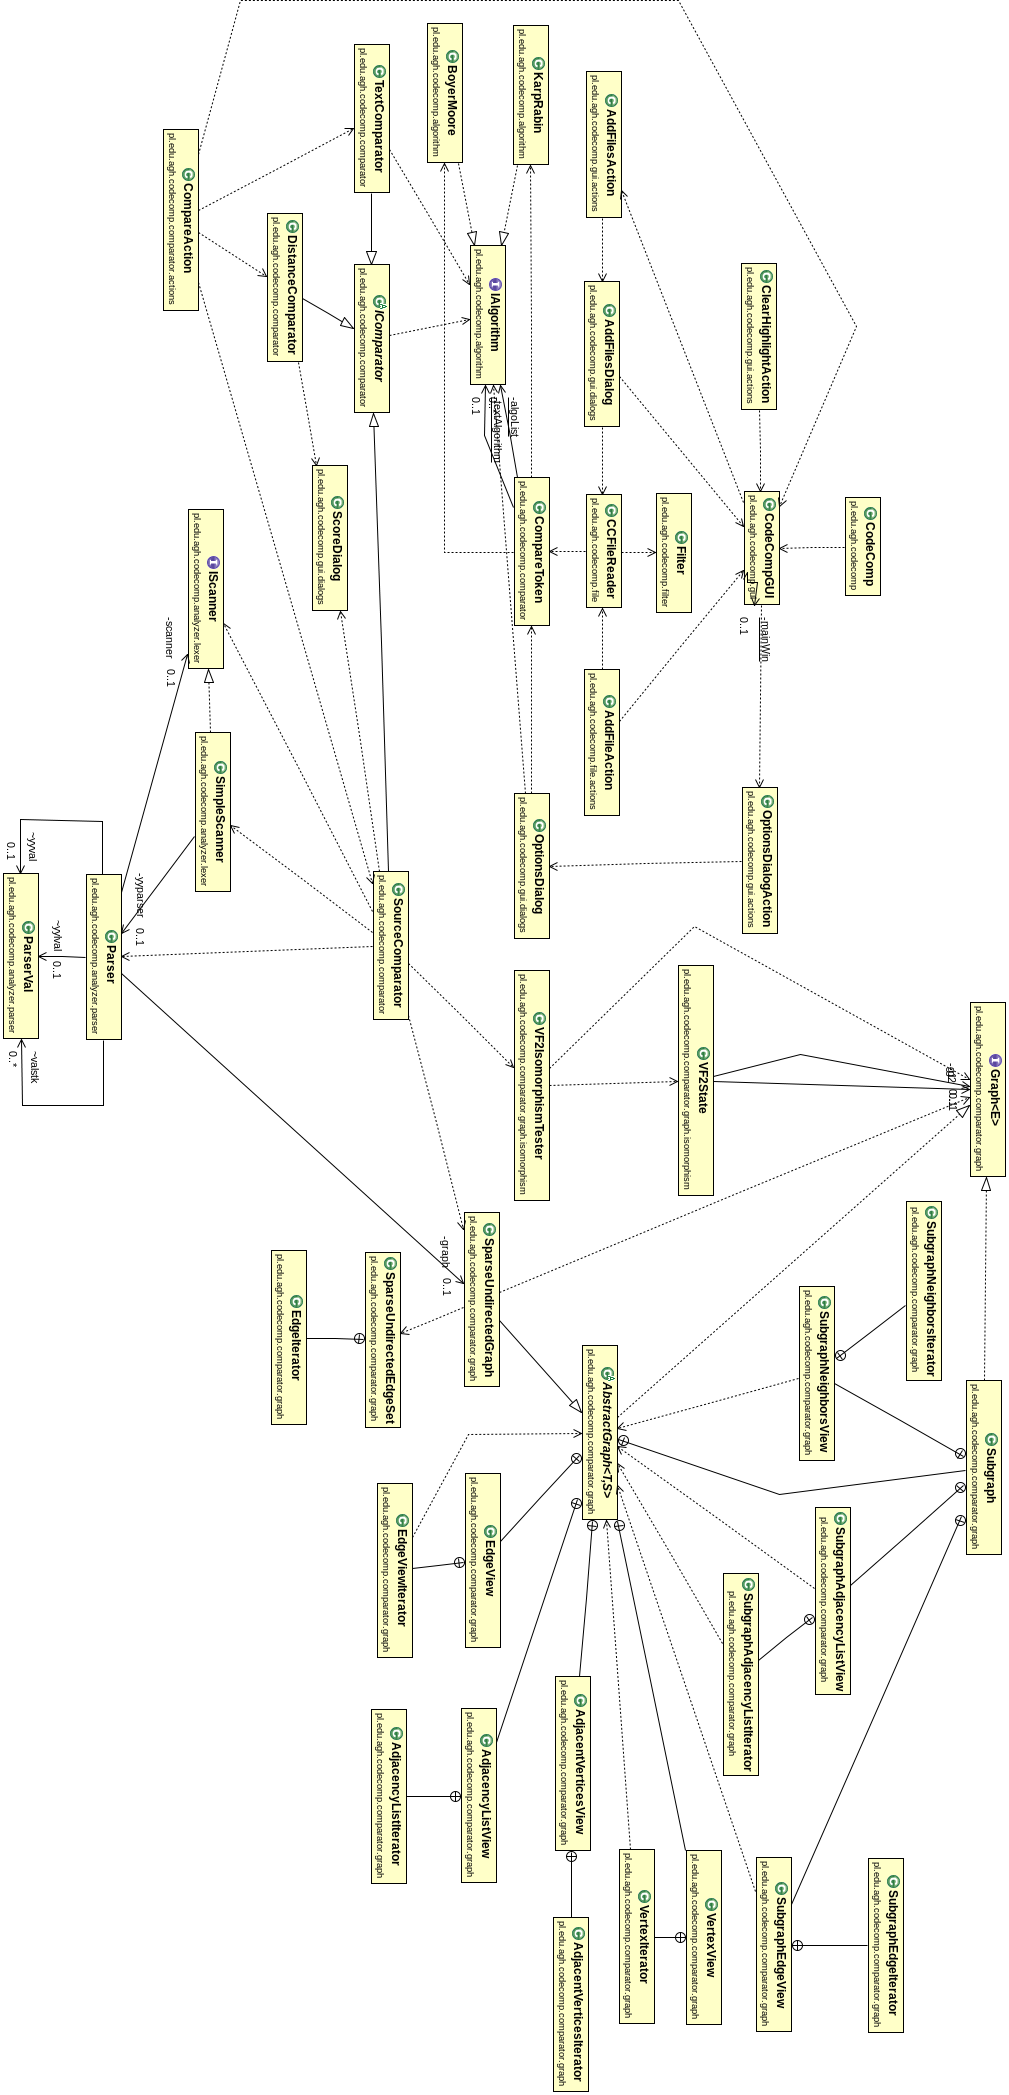
\includegraphics[scale=0.3]{gfx/ClassDiagram2.png}
\end{figure}

\pagebreak

Program posiada graficzny interfejs użytkownika stworzony za pomocą bilbioteki Swing. Składa się on z dwóch elementów tekstowych wyświetlających wczytane kody źródłowe oraz podświetlający elementy, które są identyczne/podobne. Wczytywanie oraz wszelkie inne operacje dostępne są z poziomu głównego menu znajdującego się w górnej części okna.

\begin{figure}[!h]
\centering
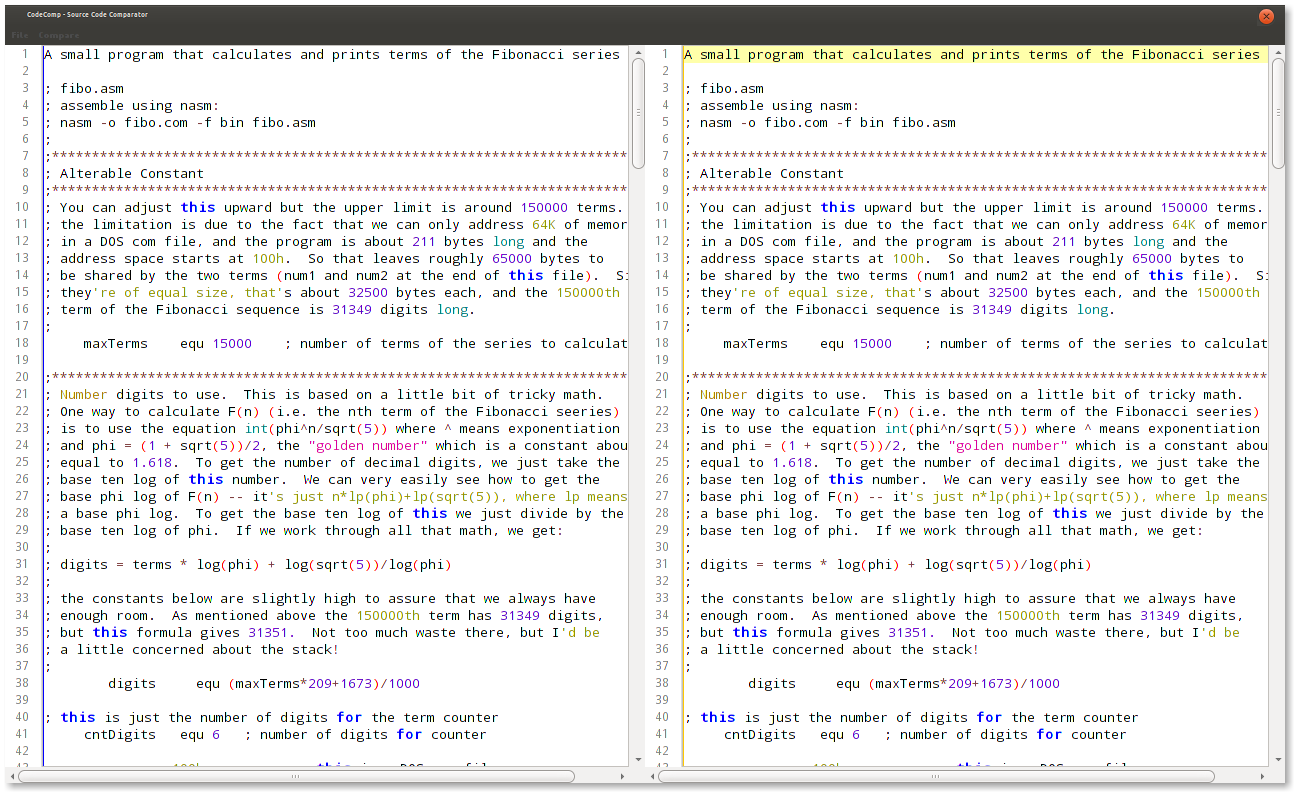
\includegraphics[scale=0.33]{gfx/main_window.png}
\end{figure}

\newpage

\subsection{Uruchamianie aplikacji}

Aplikacja dołączona do niniejszej pracy dyplomowej w całości napisana została w języku Java. Wykorzystuje ona podstawowe pakiety ze środowiska JRE 1.7 oraz kilka dodatkowych, niestandardowych bibliotek:
\begin{itemize}
\item RSyntaxArea - wykorzystywana do prezentowania kodów źródłowych
\item JFlex - odpowiada za wygenerowanie analizatora leksykalnego (skaner)
\item BYacc - odpowiada za wygenerowanie analizatora składniowego (parser)
\end{itemize}
\\ \\
Aplikacja dołączona została w postaci kodu źrodłowego oraz skompilowanego archiwum JAR, który można uruchomić na dowolnym środowisku z zainstalowanym pakietem uruchomieniowym JRE w wersji 1.7 za pomocą polecenia:
\\ \\
java -jar codecomp.jar

\newpage

\subsection{Korzystanie z aplikacji}

Po uruchomieniu aplikacji ukazuje nam się główne okno programu. Aby dodać kody źródłowe do porównania należy z głównego menu wybrać:

$\textbf{Files} \rightarrow \textbf{Add Files}$
\begin{figure}[here]
\centering
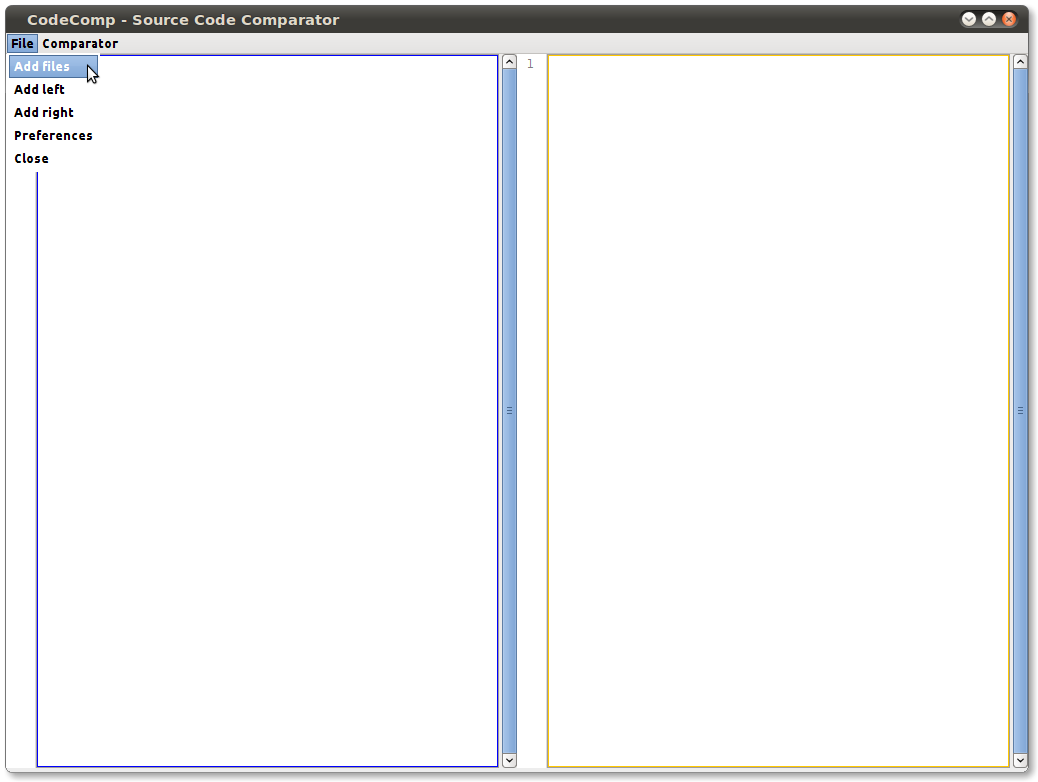
\includegraphics[scale=0.25]{gfx/add_files.png}
\caption{Okno, które ukazuje się po uruchomieniu aplikacji CodeComp.}
\end{figure}

W otwartym oknie wybieramy kody źródłowe, które chcemy porównać i klikamy $\textbf{Ok}$.
\begin{figure}[!]
\centering
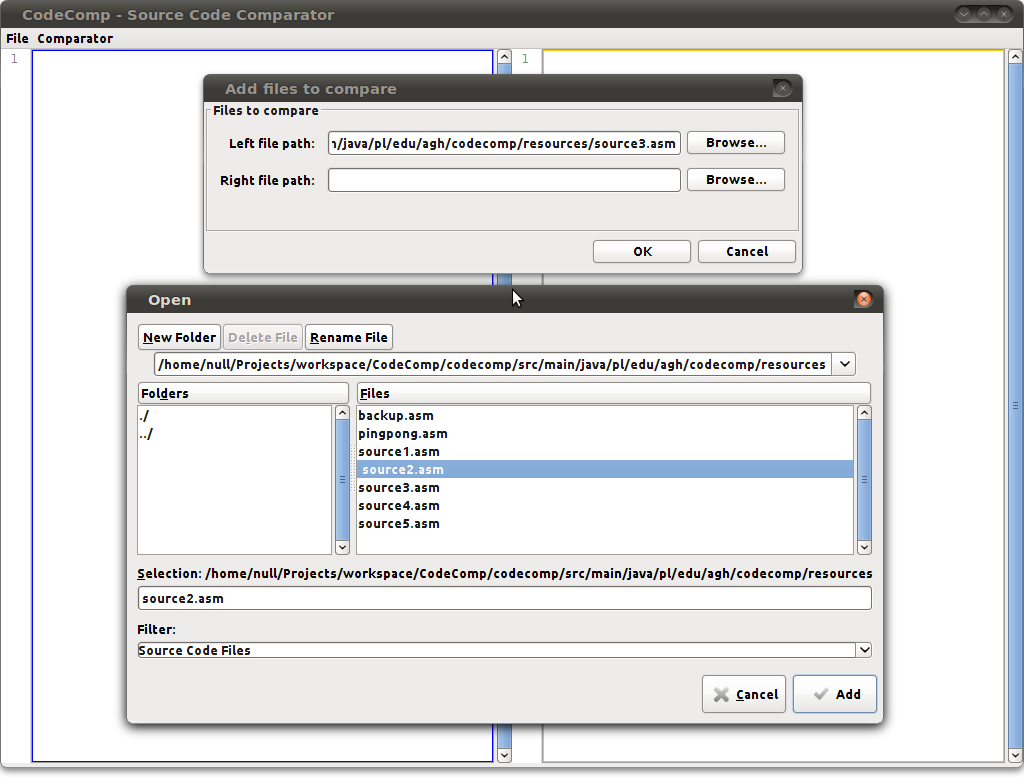
\includegraphics[scale=0.25]{gfx/select_files.png}
\caption{Wybrów plików w programie CodeComp.}
\end{figure}

\pagebreak

Następnie z menu głównego wybieramy:

$\textbf{Compare} \rightarrow \textbf{Compare source}$
\begin{figure}[here]
\centering
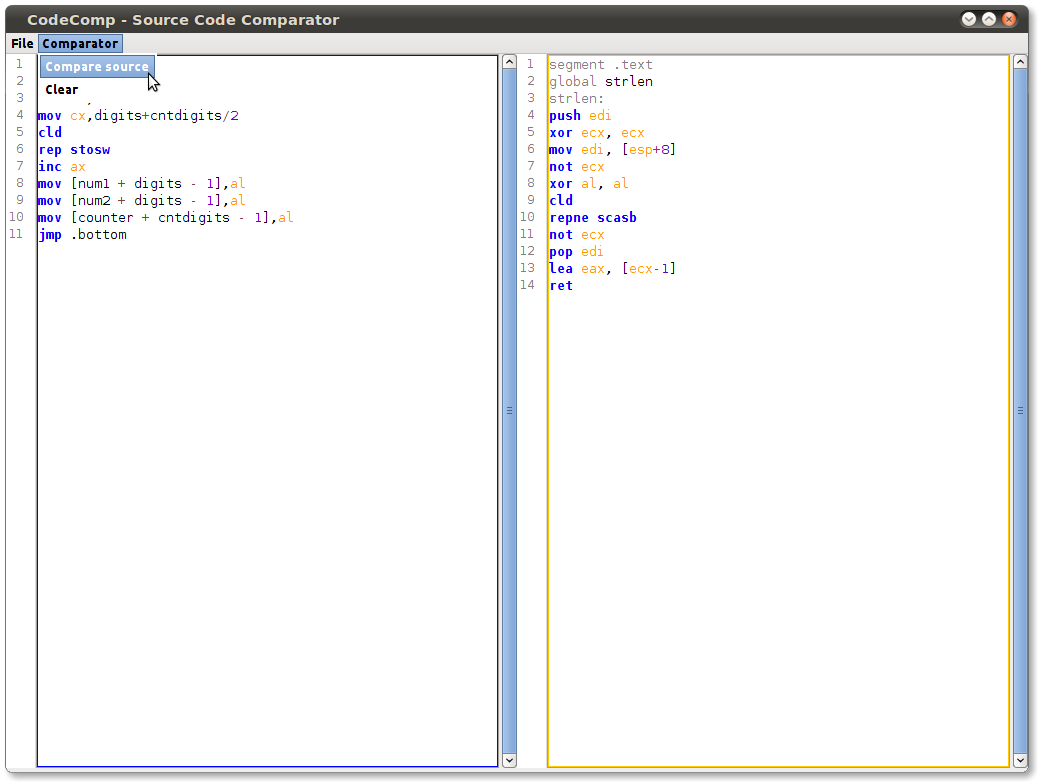
\includegraphics[scale=0.3]{gfx/compare_source.png}
\caption{Uruchomienie analizy w programie CodeComp.}
\end{figure}
\\
Wynik powinien pojawić się po chwili w osobnym oknie.
\begin{figure}[!]
\centering
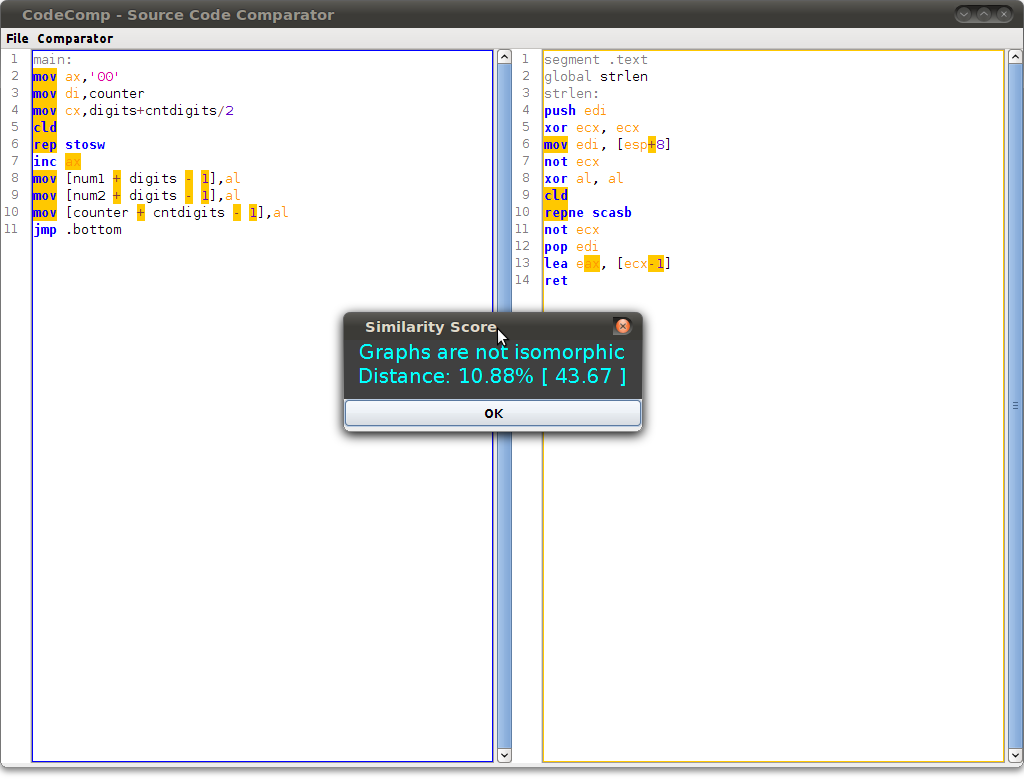
\includegraphics[scale=0.3]{gfx/compare_score.png}
\caption{Wynik działania aplikacji CodeComp.}
\end{figure}

\newpage

\subsection{Opis procesu}

\subsubsection{Preprocesing}

Pierwszym etapem całego mechanizmu powinna być faza preprocessingu, czyli odpowiedniego przefiltrowania plików źródłowych, celem usunięcia zbędnych białych znaków oraz komentarzy.

Za etap ten odpowiada Filtr, który posiada dwie funkcje: usuń białe znaki oraz usuń komentarze.

Pierwsza funkcja usuwa wszystkie białe znaki oraz usuwa puste linie. Druga funkcja usuwa wszystkie komentarze zaczynające sie od znaku średnika (\textbf{';'}) i znaku zapytania (\textbf{'?'}).

\subsubsection{Analiza}

Etap analizy dzieli się na 2 elementarne części:
\begin{itemize}
\item analizę leksykalną – wczytywanie znaków i grupowanie ich w większe symbole
\item analizę składniową – sprawdzenie poprawności z gramatyką, stworzenie drzewa składniowego 
\end{itemize}

Pierwszym krokiem jest proces analizy leksykalnej. Jej zadaniem jest wyłonienie odpowiednich symboli leksykalnych, które zostaną przekazane do analizatora składniowego.

JFlex\cite{jflex}, który został wykorzystany do stworzenia analizatora leksykalnego, generuje pliki źródłowe w języku Java na podstawie pliku specyfikacji, który składa się z trzech części:
\begin{itemize}
\item Kod użytkownika
\item Opcje i deklaracje
\item Reguły leksykalne
\end{itemize}

\pagebreak

W sekcji \textbf{Kod użytkownika} implementuje się kod, który w całości zostanie skopiowany i umieszczony w klasie wygenerowanego skanera. Zazwyczaj umieszcza się tu tylko i wyłącznie deklaracje pakietu i wymagane klasy do zaimportowania.
\\

Sekcja \textbf{Opcje i deklaracje} jest dużo bardziej złożona. Definiuje się w niej opcje generatora JFlex oraz deklaracje makr (zmiennych). Makro składa się z identyfikatora, operatora przypisania ('=') oraz wyrażenia regularnego.

\begin{figure}[here]
\centering
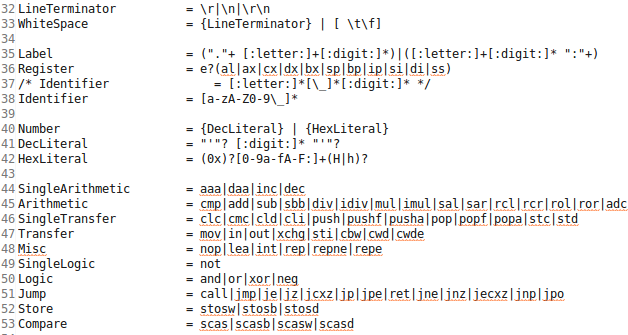
\includegraphics[scale=0.7]{gfx/regexp.png}
\caption{Lista makr zdefiniowanych w programie CodeComp.}
\end{figure}

Ostatnią częścią tej sekcji jest deklaracja stanów leksykalnych, które będą mogły być wykorzystane w następnej sekcji.
\\

\textbf{Reguły leksykalne} to sekcja, która składa sie z wyrażeń regularnych i akcji wykonywanych przez skaner po dopasowaniu wyrażenia regularnego. Podczas wczytywania danych wejściowych skaner śledzi wszystkie wyrażenia regularne i wykonuje akcję wyrażenia, które posiada najdłuższe dopasowanie. Jeśli dwa wyrażenia regularne posiadają najdłuższe dopasowanie do aktualnie przetwarzanej danej wejściowej to wykonywana jest akcja przypisana do tego, który jest zdefiniowany jako pierwszy w specyfikacji.

W przypadku aplikacji \textbf{CodeComp} wykonywane akcje przekazują do parsera zdefiniowane symbole, które będą wykorzystywane jako tokeny podczas analizy składniowej.

\begin{figure}[h]
\centering
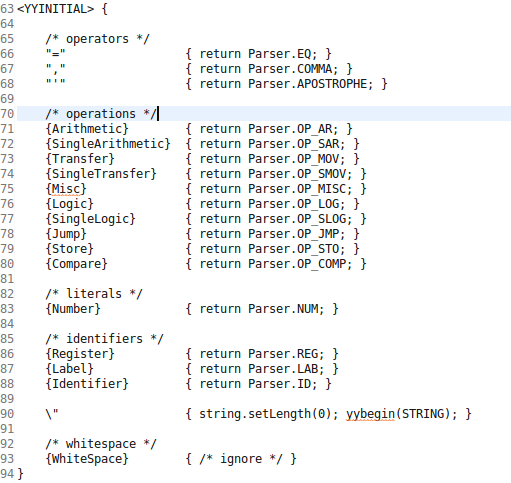
\includegraphics[scale=0.7]{gfx/actions.png}
\caption{Lista reguł leksykalnych w programie CodeComp.}
\end{figure}

Dodatkowo w tej sekcji mogą być wykorzystane stany leksykalne. Działają one jak etykiety i oznaczają, które wyrażenia regularne mogą być dopasowywane w trakcie, gdy analizator znajduje się w określonym stanie leksykalnym.
\\ \\

Kolejnym krokiem analizy jest parsowanie, które odbywa się za pomocą analizatora składniowego. Sprawdza on, czy przekazane symbole wejściowe są zgodne z gramatyką języka oraz buduje z nich graf nieskierowany, który będzie wykorzystywany podczas porównywania kodów źródłowych.

Analizator składniowy został wygenerowany za pomocą narzędzia BYacc\cite{byacc} na podstawie pliku specyfikacji, który składa się z trzech sekcji:
\begin{itemize}
\item Deklaracje
\item Reguły
\item Kod użytkownika
\end{itemize}

W sekcji \textbf{Deklaracje}, podobnie jak w przypadku analizatora składniowego, określamy pakiet projektu, w którym znajdzie się parser i importy wymaganych klas. Jednak w przypadku analizatora składniowego sekcja ta ma jeszcze inne, ważniejsze role. Oprócz wcześniej wspomnianych deklaracji określamy tutaj punkt startowy parsera oraz listę tokenów, czyli symboli obsługiwanych przez skaner.

\begin{figure}[here]
\centering
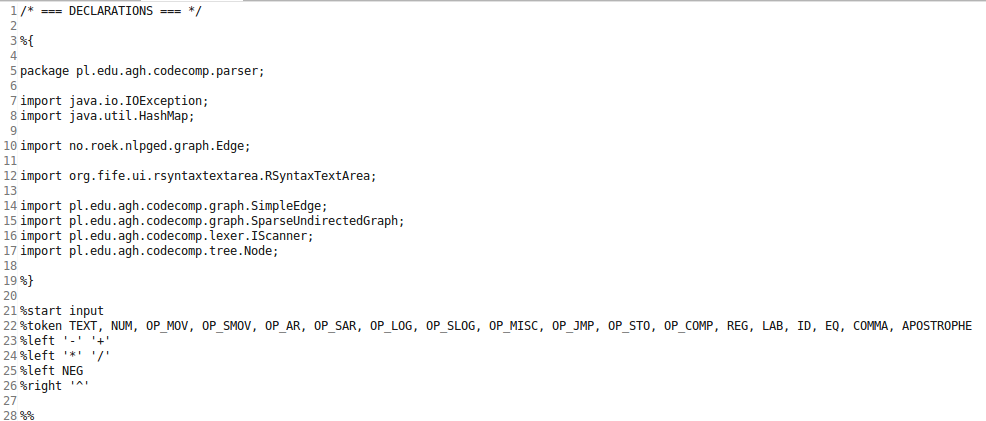
\includegraphics[scale=0.4]{gfx/parser_dec.png}
\caption{Sekcja deklaracji analizatora składniowego w programie CodeComp.}
\end{figure}
\\

Sekcja \textbf{Reguły} zawiera reguły gramatyczne, które składają się z identyfikatora, dowolnej liczby tokenów i literałów oraz przypisanej do identyfikatora akcji.

Parser na wejściu otrzymuje symbol leksykalny przekazany ze skanera i weryfikuje, czy jest on zgodny z gramatyką języka zdefiniowaną w tej sekcji. Po dopasowaniu odpowiedniej reguły parser wykonuje przypisaną do niej akcję.
\\ \\
\begin{figure}[here]
\centering
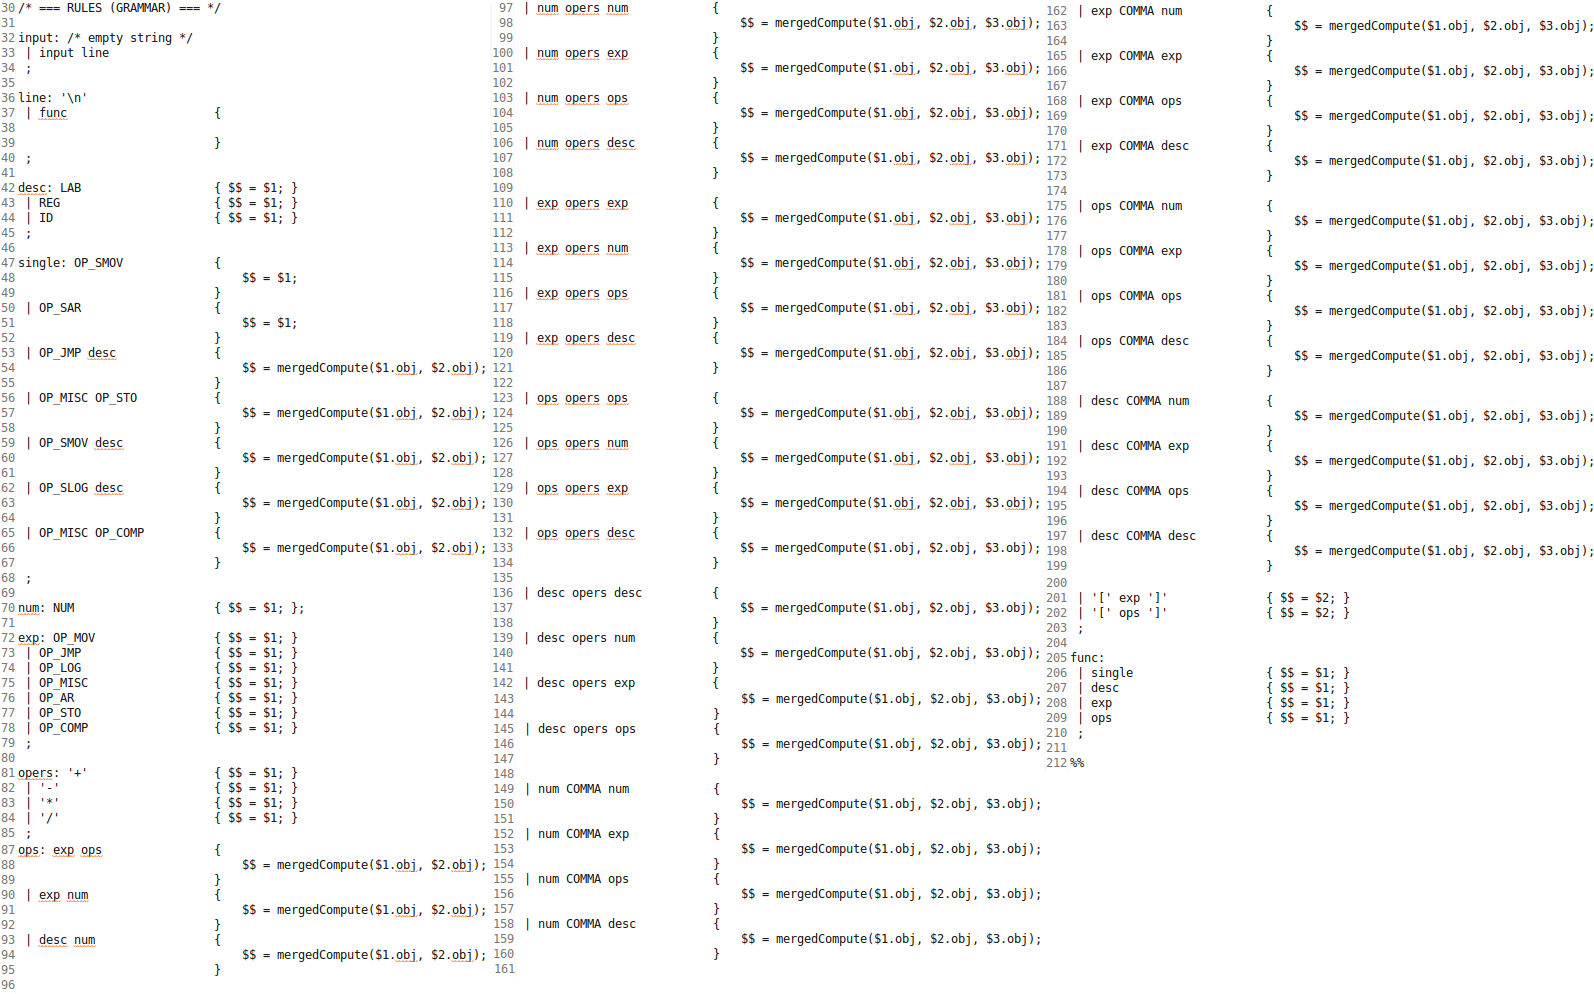
\includegraphics[scale=0.25]{gfx/parser_rules.png}
\caption{Sekcja reguł analizatora składniowego w programie CodeComp.}
\end{figure}
\\

Ostatnia sekcja - \textbf{Kod użytkownika} - jest przeznaczona na funkcje opisujące sposób parsowania oraz czynności, jakie użytkownik musi w trakcie działania parsera wykonać.

W aplikacji CodeComp zaimplementowana została funkcja, która wywołuje główną funkcję skanera zwracającą token. Następnie token ten jest przekazywany do funkcji parsujących, które sprawdzają, czy token jest zgodny z gramatyką oraz funkcji pomocniczych, które są wywoływane jako akcje reguł zdefiniowanych w poprzedniej sekcji. Funkcje pomocnicze tworzą odpowiednie węzły na podstawie wykrytych tokenów i dodają je do grafu wynikowego.

Główna funkcja parsera:
\begin{lstlisting}
private int yylex() {
 int tok = -1;
 try {
  tok = scanner.yylex();		
  Node node = new Node(yyname[tok], scanner.yytext());
  allNodes.put(node, count);
  yylval = new ParserVal(node);
  count++;
 } catch (IOException e) {
   System.err.println(e.getMessage());
 }
 return tok;
}
\end{lstlisting}
\\ \\

Funkcja pomocnicza parsera:
\begin{lstlisting}
private ParserVal mergedCompute(Node p, Node... child) {
 for(Node c : child) {
  p.addChild(c);
  graph.add(new SimpleEdge(allNodes.get(p),allNodes.get(c)));
 }
 return new ParserVal(p);
}
\end{lstlisting}
\\ \\
W aplikacji CodeComp akcje przypisane do reguł tworzą węzły i krawędzie wynikowego grafu nieskierowanego.
\\


Wynikiem wszystkich etapów analizy jest graf nieskierowany, którego węzły w sposób hierarchiczny będą przedstawiały strukturę porównywanych kodów źródłowych oraz będą przechowywać informacje na temat typów tokenów i ich wartości.

\subsubsection{Porównywanie}

\newpage

\subsection{Wyniki}

\newpage

\section{Wnioski}

\newpage

\section{Bibliografia}

\begin{thebibliography}{1}

\bibitem{arwin2006} Plagiarism Detection across Programming Languages - Christian Arwin, M.M. Tahaghoghi - Australia 2006
\bibitem{roycordy2007} Chanchal Kumar Roy and James R. Cordy - A Survey on Software Clone Detection Research - Canada 2007
\bibitem{lex} Lex - A Lexical Analyzer Generator - M. E. Lesk and E. Schmidt - http://dinosaur.compilertools.net/
\bibitem{jflex} The Fast Lexical Analyser Generator - Gervin Klein - http://jflex.de
\bibitem{lexyacc} Lex & Yacc - John R. Levine, Tony Mason, Doug Brown - O'Reilly & Associates 1992
\bibitem{byacc} BYACC/J - Tomas Hurka - http://byaccj.sourceforge.net/
\bibitem{editdistance} Binary codes capable of correcting deletions, insertions, and reversals - V. Levenshtein - Soviet Physics Doklady 1965
\bibitem{graphiso} Practical Graph Isomorphism - B.D. McKay - Congressus Numerantium,
vol. 30, pp. 45-87, 1981
\bibitem{bnf} Compiler Basics. Extended Backus Naur Form. - Farrell, James A. - 1995
\bibitem{asm_syn} Linux assemblers: A comparison of GAS and NASM - Ram Narayan - IBM Developerworks paper - 2007
\bibitem{ged} A survey of graph edit distance - Xinbo Gao, Bing Xiao, Dacheng Tao, Xuelong Li - London 2009
\bibitem{vf2} A (Sub)Graph Isomorphism Algorithm for Matching Large Graphs - Luigi P. Cordella, Pasquale Foggia, Carlo Sansone, Mario Vento - IEEE Transactions on pattern analysis and machine intelligence, vol. 26, no. 10, October 2004
\bibitem{np} Computers and Intractability: A Guide to the Theory of NP-Completeness - Michael Garey, David S. Johnson - USA 1979
\bibitem{iso_tree} P.J. Kelly, "A congruence theorem for trees" Pacific J. Math., 7 (1957) pp. 961–968; Aho, Hopcroft & Ullman 1974.
\bibitem{iso_planar} Hopcroft, J. E., John; Wong, J. (1974), "Linear time algorithm for isomorphism of planar graphs", Proceedings of the Sixth Annual ACM Symposium on Theory of Computing, 
\bibitem{iso_2} Datta, S., Limaye, N., Nimbhorkar, P., Thierauf, T., Wagner, F. (2009). "Planar Graph Isomorphism is in Log-Space". 2009 24th Annual IEEE Conference on Computational Complexity. p. 203. 
\bibitem{iso_interval} Booth, Kellogg S.; Lueker, George S. (1979), "A linear time algorithm for deciding interval graph isomorphism", Journal of the ACM 26 (2)
\bibitem{iso_perm} Colbourn, C. J. (1981), "On testing isomorphism of permutation graphs", Networks 11: 13–21
\bibitem{iso_ktree} Bodlaender, Hans (1990), "Polynomial algorithms for graph isomorphism and chromatic index on partial k-trees", Journal of Algorithms 11 (4): 631–643
\bibitem{iso_degree} Luks, Eugene M. (1982), "Isomorphism of graphs of bounded valence can be tested in polynomial time", Journal of Computer and System Sciences 25: 42–65
\bibitem{iso_genus} Miller, Gary (1980), "Isomorphism testing for graphs of bounded genus", Proceedings of the 12th Annual ACM
\bibitem{ullmann} An Algorithm for Subgraph Isomorphism - J.R. Ullmann - National Physical Laboratory, Tedd, ngton, M, ddlcsex, England 1975

\end{thebibliography}

\end{document}
